%!TEX root = ../lectures_olympics.tex

\chapter{微积分在物理当中的应用}


在过去的学习中我们已经学了很多的物理定律以及它们的应用,对于一大类问题来说可以通过已知的定律结合系统地分析已经能够完成,其中也包括一些非常基本和复杂的问题。
但在学习过程中同学们一定发现在处理一些问题的时候会遇到一定程度上数学的困难,甚至从学习运动的第一天开始就普经提到过,位置随时间的变化率被定义为速度,而我们其实还没有掌握对于任意给定的运动而求出其速度的普遍方法,只是对于一部分非常常见的运动形式用其它方法得到其速度与时间的关系;
此外还曾提到,速度-时间图像与横轴在两条垂直于时间轴的线所围成的面积就是在给定时间里运动质点的位移,但也无法对于一般的速度通过定义求出任意一段时间里的位移。
在历史上人们在试图理解引力以及引力的性质时也遇到了类似的情况,相信结果大家都很有所耳闻,牛顿({\it I. Newton})和莱布尼茨({\it G. W. Leibniz})分别独立地发明了一种全新的数学工具---{\heiti 微积分}(calculus)而使处理类似的问题有了可能。
微积分,以及随之而来的一整套数学理论极大地推动了物理学的发展,不但能够使我们能够处理很多和曲线、曲面性质相关的物理问题,其中也包含着重要的物理思想。

\section{导数及其应用}

具有光滑图像的单自变量函数在各个点上切线的斜率称为函数的{\heiti 导函数}(derivative)。
如果将函数记做$y = y(x)$,它的图像在某一$x$点处切线可以看做割线的极限,其斜率为
\begin{equation}\label{key}
\lim_{x\rightarrow 0}\frac{y(x+\Delta x)-y(x)}{\Delta x},
\end{equation}
导函数有很多表示方法,例如$y'(x)$、$\frac{dy}{dx}(x)$都是常见的形式。
在物理当中会遇到的绝大部分函数都可以进行{\heiti 求导运算}(differentiation),除了计算出特定函数的导数以外还需要充分地了解其物理意义。

例如直线运动质点的速度就是其坐标对时间的导数:
\begin{equation}\label{key}
v(t) = \frac{dx}{dt}(t),
\end{equation}
类似地加速度是速度对时间的导数:
\begin{equation}\label{key}
a(t) = \frac{dv}{dt}(t).
\end{equation}
从中还可以看出加速度实际上就是坐标对时间导数的导数,我们称它为坐标对时间的{\heiti 二阶导数}(second order derivative),记做$x''$或$\frac{d^2x}{dt^2}$。
类似地还可以定义更高阶的导数。

很多物理量都是借助导数而定义的,只是由于在我们目前所处理的绝大部分问题当中为了简单起见没有指明而已。
例如对于一根具有弹性的绳,实验上能够进行测量的实际上是它的形状量和所受外力的关系,如果将形变量记做$x$、所受外力记做$F$的话实验给够给出函数$F(x)$。
弹性系数可以看成是当弹簧已经处于某一形变$x$时,为了再拉开$\Delta x$的长度所需要增加的外力,如果弹簧满足胡克定律的话,弹性系数是一个常数,对于一个一般的弹性体而言,其弹性系数有可能随形变量的改变而改变:
\begin{equation}\label{key}
k(x) = \frac{dF}{dx}(x).
\end{equation}
与之类似地,实验上可以测量在特定条件下从某一温度开始一个给定物体所吸收热量和温度的关系$Q(T)$,比热是当它处于某一温度时当温度再升高$\Delta T$所需要的热量,根据导数的定义可知
\begin{equation}\label{key}
c(T) = \frac{dQ}{dT}(T),
\end{equation}
除非是理想气体,对于任何真实物体而言其比热都是温度的函数。

利用导数的定义以及一些基本的运算法则就可以得到物理当中所遇到的绝大部分函数的导数。
接下来通过一些具体的例子来熟悉一下基本的求导运算规律。

%%%%%%%%%%%%%
\begin{example}
	根据定义求下列函数的导数:
	\[
	y(x) = C,\qquad y(x) = kx,\qquad y(x) = ax^n, \qquad y(x) = A\sin(kx),\qquad y(x) = e^{x}
	\]
	其中除了已经明确给出的自变量$x$以外都是常数。
	\tagged{student}{\vspace*{4cm}}
	\begin{taggedblock}{teacher}
		\newline
		解析:1.0  2.
	\end{taggedblock}
\end{example}
%%%%%%%%%%%%%%%%%%%%

%%%%%%%%%%%%%
\begin{example}
	函数$f(x)$、$g(x)$对$x$的导数为已知,根据导数的定义证明以下几个求导运算的基本规律:
	\begin{eqnarray*}
		\frac{d}{dx}[af(x)] &=& a \frac{df}{dx}(x)\\
		\frac{d}{dx}[f(x)g(x)] &=& f\frac{dg}{dx}+\frac{df}{dx}g\\
		\frac{d}{dx}f(g(x)) &=&\frac{df}{dg}\frac{dg}{dx}\\
	\end{eqnarray*}
	\tagged{student}{\vspace*{4cm}}
	\begin{taggedblock}{teacher}
		\noindent
		解析:略
	\end{taggedblock}
\end{example}
%%%%%%%%%%%%%%%%%%%%


\subsection{物理量的变化率}

导数在物理中最为直接的应用莫过于求出一个物理量对另一个物理量的变化率,这一计算广泛地存在于物理学的各个地方。
例如前面提到过的速度就是坐标随时间的变化率,加速度是速度随时间的变化率,保守力的大小也与势函数随坐标的变化率有着直接的关系。
有些时候可以直接写出两个物理量之间的函数关系,这时它们之间的关系非常清楚,直接求导就可以得到在一个物理量发生变化时另一个物理量的变化率。

%%%%%%%%%%%%%%%
\begin{example}
	一个一维运动质点的坐标随时间的关系为以下已知函数时,求瞬时速度、加速度与时间的函数:
	
	1. $x(t) = v_0 t+\frac{1}{2}at^2$;
	
	2. $x(t) = Ae^{-\beta t}\cos(\omega t)$,$\beta$,$\omega$为已知数;
	
	3. $x(t) = \frac{mv_0}{\beta}\left[1-e^{-\frac{\beta}{m}t}\right]$,其中$\beta$、$m$为已知数。
	\tagged{student}{\vspace*{4cm}}
	\begin{taggedblock}{teacher}
		\newline
		解析:1.$v=v_0+at,a=a$
		\\2.$v=-Ae^{-\beta t}[\omega\sin(\omega t)+\beta\cos(\omega t)],a=Ae^{-\beta t}[2\beta\omega\sin(\omega t)+\beta^2\cos(\omega t)-\omega^2\cos(\omega t)]$
		\\3.$v=v_0e^{-\frac{\beta}{m}t},a=-\frac{\beta v_0}{m}e^{-\frac{\beta}{m}t}$
	\end{taggedblock}
\end{example}%%%
%%%%%%%%%%%%%%$$

%%%%%%%%%%%%%%%
\begin{example}
	一个半径为$R$的半圆柱体在垂直于柱轴水平方向上以匀速$v_0$运动,如图所示在圆柱面上搁一竖直杆,此杆只能沿竖直方向上下运动。
	求杆上任意一点速度和与加速度与由图中给出的角度$\theta$的关系。
	\begin{flushright}
		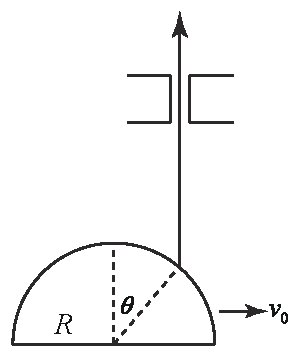
\includegraphics[width = 0.3\textwidth]{images/motion-44.pdf} 
	\end{flushright}
	\tagged{student}{\vspace*{1cm}}
	\begin{taggedblock}{teacher}
		\noindent
		解析:$v=v_0\tan\theta,a=\frac{v_0}{R\cos^3\theta}$
	\end{taggedblock}
\end{example}%%%
%%%%%%%%%%%%%%$$


%%%%%%%%%%%%%%%
\begin{example}
	一个发光点在焦距为$f$的凸透镜主光轴上以恒定不变的速度$v$向着透镜运动,求其像点移动的速度与物距$u$的关系。
	\tagged{student}{\vspace*{4cm}}
	\begin{taggedblock}{teacher}
		\newline
		解析:$v'=-\frac{f^2v}{u-f}$
	\end{taggedblock}
\end{example}%%%
%%%%%%%%%%%%%%$$

\subsection{求极值}
对于一个光滑的函数来说,当其自变量发生变化时函数值连续变化,一般来说其各点的切线方向也做不断地变化,我们知道函数光滑的曲线上每一点的切线的斜率就是函数在该点的导数。
通过对函数图像的观察不难发现,当它在某一点处的切线为水平时,定性地看函数的图像可能有如图所示的三种情况,对于前两种情况,切线为零点处的函数值都一致地大于或小于周围点处的值,我们称它们为函数的{\heiti 局部极大值}(local maximum)或{\heiti 局部极小值}(local minimum),合称{\heiti 局部极值}(local extreme)。第三种情况比较特殊,当把它周围的图像放大后仔细观察可以发现,其图像在该点处既不是极大也不是极小,但在该处很接近这一点处的水平切线,称为稳定点。
无论哪种情况,当函数在某点处的导数值为零时,都称这样的点为函数的{\heiti 稳定点}(stationary point),有三种可能的稳定点,分别为局部极大、极小值或非极值的稳定点。
极值点的位置由一阶导数为零给出,到底是哪种类型的极值点则需要利用函数的二阶导数在极值点处的符号来确定,二阶导数为正,则是局部极小值;二阶导数为负则是局部极大值;二阶导数为零则需要做进一步的判断。
\begin{figure}[hbtp]
\centering
\includegraphics[width=0.9\textwidth]{images/cal-1.pdf}
\caption{函数的导数为零的各种情况}
\end{figure}

当一个感兴趣的物理量随着其它因素发生变化时,找到它们之间的依赖关系,求出它们的导数,导数为零的点就是该物理量在变化过程当中的极值点。
如果对该极值点到底为哪种类型的极值点时,就需要进一步求出函数在该点的二阶导数并根据其正负来确定。
以下就是一些典型的例子。
\begin{example}
利用费马原理证明光的折射定律:设有两个均匀介质其折射率分别为$n_1$和$n_2$,它们之间的分界面为一平面。
试证明由平面外任意一点$A$发出的到达$B$的光线当中满足折射定律的光线的光程为极值。
\begin{flushright}
\includegraphics[width=0.3\textwidth]{images/cal-2.pdf} 
\end{flushright}
\tagged{student}{\vspace*{2cm}}
\begin{taggedblock}{teacher}
\noindent
解析:从A到B经过P点的光线的光程与$x$的关系为
\[L=n_1\sqrt{x^2+h_1^2}+n_2\sqrt{(L-x)^2+h_2^2}\]
它取极值的条件为
\[
\frac{dL}{dx} = n_1\frac{x}{\sqrt{x^2+h_1^2}}-n_2\frac{L-x}{\sqrt{(L-x)^2+h_2^2}}=n_1\sin\alpha-n_2\sin\beta=0,
\]
折射定律自然得证。
\end{taggedblock}
\end{example}



\begin{example}
求理想气体在下面两个热力学过程当中温度的最大值和最小值:

(a)$p-V$图中的一条直线,通过$(2p_0,V_0)$和$(p_0,2V_0)$两点;

(b)$p-V$图中的一个圆(椭圆),过程满足\[(\frac{p}{p_0}-1)^2+(\frac{V}{V_0}-1)^2=\left(\frac{1}{2}\right)^2\]
\begin{center}
\includegraphics[width=0.7\textwidth]{images/cal-3.pdf} 
\end{center}
\tagged{student}{\vspace*{4cm}}
\begin{taggedblock}{teacher}
\noindent
解析:第一个过程,压强和体积的关系为\[p=3p_0-\frac{p_0}{V_0}V,\]
根据理想气体的状态方程,温度和体积的关系可以写为
\[
T=\frac{1}{nR}(3p_0-\frac{p_0}{V_0}V)V
\]
这样温度取极值的条件为:
\[
\frac{dT}{dV} = \frac{1}{nR}(3p_0-\frac{p_0}{V_0}V-\frac{p_0}{V_0}V)=0
\]
很容易得到其解为$V=\frac{3}{2}V_0$,根据状态方程可得该点的温度
\[
T=\frac{1}{nR}\frac{3}{2}p_0\frac{3}{2}V_0 = \frac{9}{4}\frac{p_0V_0}{nR} = \frac{9}{8}T_0
\]
其中$T_0$为气体在A或B点的温度,从中也可看出温度极值为最大值。

对于第二个问题也类似,但压强与体积的关系比较复杂,为此采用参数化的方法,设循环过程上的点和中心$(p_0,V_0)$点连线与横轴的夹角为$\theta$,这样各点的压强和体积可以写为
\[
\frac{p}{p_0}=1+\frac{1}{2}\sin\theta,\qquad \frac{V}{V_0}=1+\frac{1}{2}\cos\theta,
\]
这样温度和角度$\theta$之间的关系可写成
\[
T=\frac{1}{nR}pV = \frac{p_0V_0}{nR}(1+\frac{1}{2}\sin\theta)(1+\frac{1}{2}\cos\theta)
\]
这时温度取极值的条件$\frac{dT}{d\theta}=0$可以化为如下方程:
\[
-\frac{1}{2}\sin\theta(1+\frac{1}{2}\sin\theta)+\frac{1}{2}\cos\theta(1+\frac{1}{2}\cos\theta)=0
\]
化简整理可得
\[
(\cos\theta-\sin\theta)(\cos\theta+\sin\theta+2)=0
\]
上式的解只能是$\sin\theta=\cos\theta$,也就是$\theta = 45^\circ,225^\circ$。

\end{taggedblock}
\end{example}



\begin{example}
宇宙中有两个天体质量均为$M$,相距$2L$,求在它们连线的垂直平分线上何处的小天体受到两个大天体万有引力能够达到最大值。
\begin{flushright}
\includegraphics[width=0.3\textwidth]{images/cal-4.pdf} 
\end{flushright}
\tagged{student}{\vspace*{1cm}}
\begin{taggedblock}{teacher}
\noindent
解析:本题比较直接,当另一天体所处的位置如图所示时,它与两个天体之间连线中点的距离为$x$,那么小天体受到的引力
\[
F = 2G\frac{M^2}{L^2+x^2}\frac{x}{\sqrt{L^2+x^2}} = 2GM^2\frac{x}{(L^2+x^2)^{3/2}},
\]
将引力对$x$求导可得
\[
\frac{dF}{dx}=2GM^2[\frac{1}{(L^2+x^2)^{3/2}}-\frac{3x^2}{(L^2+x^2)^{5/2}}]=2GM^2\frac{L^2-2x^2}{(L^2+x^2)^{5/2}},
\]
这样引力取最大值的条件为$x=\pm L/\sqrt{2}$。
进一步可以求出最大的引力值为
\[
F_{max} = 2\frac{GM^2}{L^2}\frac{1}{\sqrt{2}\cdot (\frac{3}{2})^{3/2}}
\]
\end{taggedblock}
\end{example}


\begin{example}
(a) 如图所示的坐标系原点处以给定初速度$v_0$沿不同角度抛出物体,它能够击中一些目标,但对于那些很高或很远的目标则由于初速度不够而无法击中,求证这两类目标分界线所满足的方程
\[y=\frac{v_0^2}{2g}-\frac{g}{2v_0^2}x^2\]
(b) 如图所示平面上有一个半径为$R$的球体,我们希望在地面上斜向上抛出一个物体击中球体的顶部。
求在不碰到球体的条件下能够击完成目标的最小的抛出速度$v_{min}$、抛出的角度$\theta_0$以及抛出点与球底部的距离$d_0$。
%\begin{flushright}
%\includegraphics[width = 0.3\textwidth]{images/抛向一个球顶的球.pdf} 
%\end{flushright}

\tagged{student}{\vspace*{4cm}}
\begin{taggedblock}{teacher}
\noindent
解析:在标准的坐标系当中,以速度$v_0$,角度$\theta$抛体的轨迹方程满足
\[y=\tan\theta x-\frac{gx^2}{2v_0^2\cos^2\theta},\]
对于给定的水平位置$x$,它所能够打到最高点对应的抛出角度可由上式对$\theta$求导后对于给定的$x$导数值为零所对应的角度所给出。
通过观察可以发现上式右边第二项实际上可以表达为$\frac{1}{\cos^2\theta}=1+\tan^2\theta$,所以轨迹方程实际上可以看成是$u=\tan\theta$的方程更为简单一些。
导数为零的条件为
\[
\frac{dy}{d(\tan\theta)}=x-\frac{gx^2}{v_0^2}\tan\theta=0
\]
从它出发可以解出
\[
\tan\theta = \frac{v_0^2}{gx}
\]
这样抛体在$x$处所能够达到的最大高度为
\[
y_{max} = x\frac{v_0^2}{gx}-\frac{gx^2}{2v_0^2}(1+\frac{v_0^4}{g^2x^2}) = \frac{v_0^2}{2g}-\frac{g}{2v_0^2}x^2.
\]

第二问要复杂一些,根据抛体运动的可逆性,从地面抛出的物体如果能够击中顶部的话,以相反的速度从顶部抛出则可沿着相同的轨迹落到地面,根据能量守恒,顶部抛出物体的速度越小则到达地面时的速度就越小。
这样问题就反过来变成了从顶部抛出物体,不碰到球体表面而落到地面的最小速度。
利用前一问的答案,抛体能够打到的范围是一个随着初速度增加越来越大的抛物线,初速度不够时抛物线总会和圆有交点,这样抛体无论初速度方向如何都会碰到球。
当抛物线大到能够和球相切时就有一个可能性使沿特殊的角度抛出以后它的轨迹能够与球相切,这是不碰到球的临界条件。
当包络线与圆相切时,包络面的方程和圆的方程联立时只有一个解,当速度更大时则没有解,所以可以由这个条件解出相切对应的最小速度。
两个方程分别为
\[
y=2R+\frac{v_0^2}{2g}-\frac{g}{2v_0^2}x^2 \qquad 和\qquad
x^2+(y-R)^2=R^2
\]
注意第一个方程当中坐标系原点的变化,现在抛出点位于球的顶部,所以需要将包络线上移$2R$。
联立以后可以看做是$x^2$的一元二次方程:
\[
\frac{g^2}{4v_0^4}(x^2)^2 +\left [ 1-\frac{g}{v_0^2}(\frac{v_0^2}{2g}+R) \right ]x^2+\left [  (\frac{v_0^2}{2g}+R)^2-R^2 \right ]=0
\]
其判别式为零的条件为
\[
\Delta =(\frac{1}{2}+\frac{gR}{v_0^2})^2-4\frac{g^2}{4v_0^4}(\frac{v_0^4}{4g^2}-\frac{v_0^2R}{g})=0
\]
化简之后可以解出此时速度需要满足的条件,也就是最小的可能“击中”的速度值:
\[
v_0^2 = \frac{1}{2}gR
\]
由机械能守恒可知地面的最小抛出速度为
\[
v_{min}^2=\frac{1}{2}gR+4gR = \frac{9}{2}gR
\]
其抛出点的其它性质可由轨道给出。



\end{taggedblock}
\end{example}

\subsection{求稳定点和稳定性}
正所谓“人往高处走,水向低处流”,自然界中的任何物体都有向着能量最低的的状态运动的趋势,加上它们自身的惯性决定了所有物质的运动方式。
这样当一个物理系统处于静止或平衡状态时,它一定对应着所有能量取极小值或局部极小值。
过去我们判断物理系统平衡状态往往采用基于系统内部物体受力的分析,其实通过其能量为极小值也能够得到相同的答案并且具有更广泛的应用范围,经验表明:越复杂的物理系统,利用能量取极小这个条件往往能够更容易地找到其平衡或稳定状态。

\begin{figure}[hbtp]

\begin{minipage}[t]{0.5\linewidth}
\centering
\includegraphics[width = 0.3\textwidth]{images/cal-6.pdf}
\caption{}\label{fig: 微积分,摆的稳定性}
\end{minipage}
\begin{minipage}[t]{0.5\linewidth}
\centering
\includegraphics[width=0.8\textwidth]{images/cal-7.pdf} 
\caption{}\label{fig: 微积分,任意势能下的稳定性}
\end{minipage}

\end{figure}

以最简单的摆为例,如图\ref{fig: 微积分,摆的稳定性}所示一根长度为$l$,质量忽略不计的刚性杆一端与$O$点光滑连接,另一端连接一个质量为$m$的质点,这个系统的重力势能与它的摆动角度$\theta$之间有简单的关系
\begin{equation}
E_p = -mgl\cos\theta,
\end{equation}
这样其势能取极值的条件是它对角度的导数为零:
\begin{equation}
\frac{dE_p}{d\theta}=mgl\sin\theta,
\end{equation}
数学上当$\theta =0,\pi$时导数为零,分别对应于摆竖直向下和竖直向上两种情况。
很明显只有当$\theta=0$的点为它的稳定平衡点,$\theta=\pi$处为不稳定的平衡点,虽然该点处受力平衡,但在任意微小的扰动下该平衡状态必将被打破。
这一点也可以由势能对角度的二阶导数
\begin{equation}
\frac{d^2E_p}{d\theta^2} = mgl\cos\theta
\end{equation}
的正负很容易地看出。
$\theta=0$时$\frac{d^2E_p}{d\theta^2} = mgl>0$,为稳定平衡点,$\theta=\pi$时$\frac{d^2E_p}{d\theta^2} =- mgl<0$,表现为不稳定平衡。
更一般地,当系统的势能在某一变量的变化下的函数图像如图\ref{fig: 微积分,任意势能下的稳定性}所示时,$S_1$、$S_2$为稳定平衡点,$U_1$、$U_2$为不稳定点,$P$点也不可能平衡,数学上对应于势能的二阶导数为零的那些点。

\begin{example}
如图所示在固定点A上系有一个质量可以忽略不计,原长为$h$,劲度系数为$k$的弹簧,另一端系有一个质量为$m$的重物。
重物被限制在竖直的光滑直线上,A点距离该约束直线的距离就是它的原长$h$,求平衡时重物距离B点的距离$x$。
\begin{flushright}
\includegraphics[width=0.3\textwidth]{images/cal-8.pdf} 
\end{flushright}
\tagged{student}{\vspace*{4cm}}
\begin{taggedblock}{teacher}
\noindent
解析:取B点的重力势能为零,整个力学系统当中包含的势能有重物的重力势能和弹簧的弹性势能,它们都随着$x$的变化而变化。
当系统处在如图所示的位置时,势能为
\[E_p = -mgx+\frac{1}{2}k(\sqrt{h^2+x^2}-h)^2\]
平衡位置由势能对$x$的导数为零给出:
\[\frac{dE_p}{dx}=-mg+2k(\sqrt{h^2+x^2}-h)\frac{x}{\sqrt{x^2+h^2}}=0\]
从中解出$x$即可。
虽然$x$不容易求解,但是从中可以发现由势能为零得到的结果和静力学分析的结果完全一致。
\end{taggedblock}
\end{example}


\begin{example}
如图所示的一个锥角为$\alpha$的光滑圆椎体上放着一段质量为$m$、弹性系数为$k$、原长为$L_0$的弹簧,弹簧时刻保持水平。
试求平衡时弹簧与椎体顶端的距离$x$。
\begin{flushright}
\includegraphics[width = 0.2\textwidth]{images/cal-9.pdf} 
\end{flushright}
\tagged{student}{\vspace*{1cm}}
\begin{taggedblock}{teacher}
\noindent
解析:弹簧的重力+弹性势能随$x$变化的关系很简单,为
\[E_p=-mgx+\frac{1}{2}k(2\pi x\tan\alpha-L)^2\]
在$x$变化的范围内它取极值的条件为
\[\frac{dE_p}{dx}=-mg+2\pi k\tan\alpha(2\pi x\tan\alpha-L)=0\]
很容易解出
\[
x = \frac{mg+2\pi k L\tan\alpha}{4\pi^2 k \tan^2\alpha}
\]
\end{taggedblock}
\end{example}

\begin{example}
如图所示的两根质量可以忽略不计、长度为$l$的杆顶部无摩擦地连接,并有一质量为$m$的重物$A$放置于两杆连接处。
其底部放在光滑的水平地面上,之间由原长为零、劲度系数为$k$的弹簧连接,求平衡时两杆与地面的夹角$\theta$。
\begin{flushright}
\includegraphics[width=0.3\textwidth]{images/cal-10.pdf} 
\end{flushright}
\tagged{student}{\vspace*{3cm}}
\begin{taggedblock}{teacher}
\noindent
解析:本题可用静力平衡来解,担很容易得到错误的结果,用能量的分析会好很多。
在角度为$\theta$时,整个系统的总的势能由重物的重力势能和弹簧的弹性势能够成:
\[E_p = mgl\cos\theta +\frac{1}{2}k(2l\sin\theta)^2 = mgl\cos\theta +2kl^2\sin^2\theta \]
这样可能的平衡位置就由势能对角度的导数为零所给出:
\[\frac{dE_p}{d\theta} = -mgl\sin\theta + 4kl^2\sin\theta\cos\theta = 0 \]
上式有两个可能的解:$\theta = 0$或者$\cos\theta = \frac{mg}{4kl}$。
为了判断平衡的稳定性,需要计算其二阶导数:
\[
\frac{d^2E_p}{d\theta^2} = -mgl\cos\theta + 4kl^2(\cos^2\theta-\sin^2\theta)
\]
对于$\theta=0$的解,我们有
\[
\frac{d^2E_p}{d\theta^2}(\theta=0) = -mgl+4kl^2
\]
可见当$k>\frac{mg}{4l}$时,二阶导数大于零, 是一个稳定的平衡状态,反之当$k<\frac{mg}{4l}$平衡不稳定。
而对于$\theta=\cos^{-1}\frac{mg}{4kl}$的解,它所对应的二阶导数值
\[
\frac{d^2E_p}{d\theta^2}=4kl^2(\frac{m^2g^2}{16k^2l^2}-1)<1
\]
一定是个不稳定的解,现实中该系统不可能平衡在任何$\theta\neq 0$的状态下!
\end{taggedblock}
\end{example}






\subsection{做展开}
如图所示,在坐标系中有一个光滑函数的图像,直线$PQ$为曲线上$P$点的切线。
仔细地观察在$P$点附近函数曲线与切线容易发现它样在$P$点附近实际上非常接近,而且对于那些与$P$点自变量非常接近的点,切线上的值与函数本身的取值的差别就越小。
这样我们就能够得到一个利用函数在一点上切线的值近似地代表函数值的手段,这种操作在物理上非常常用和有效。
函数$f(x)$在某一给定点$x_0$处的取值为$f(x_0)$,在该点处切线的斜率为其导数在$x_0$处的取值$\frac{df}{dx}(x_0)=f'(x_0)$,这样通过函数曲线在$x_0$处的切线方程就可以写成
\begin{equation}
y = f(x_0)+f'(x_0)(x-x_0)
\end{equation}
这样当$x$与$x_0$非常接近时就可以将函数值近似地表达为
\begin{equation}
f(x)\simeq y  = f(x_0)+f'(x_0)(x-x_0)
\end{equation}
当$x$与$x_0$的差别越来越小,用切线来代表曲线的近似程度就越来越高。
如果用$\Delta f$代表函数在$x_0$附近的值与$f(x_0)$的差$\Delta f = f(x)-f(x_0)$,同时令$\Delta x = x-x_0$为自变量的差值,那么上式又可以写为
\begin{equation}
\Delta f = f'(x_0)\Delta x
\end{equation}
从中可以看出对于连续函数某一给定点附近的函数值的差别正比于自变量的差别,其比例系数为函数在该点处的导数值。

实际上这样的操作在过去已经多次使用,如果用$\Delta x$代表一个远远小于1的正数,一些常见的小量展开的例子如
\begin{enumerate}
\item $\sin \Delta x\simeq\tan \Delta x\simeq  \Delta x$
\item $(1+\Delta x)^n\simeq 1+n\Delta x$
\item $e^{\Delta x}\simeq 1+\Delta x$
\item $\ln (1+\Delta x)\simeq \Delta x$
\end{enumerate}
它们在$x\rightarrow 0$时原来函数的值都非常接近,可以用展开式来近似地表示函数值。
利用小量展开在研究物理系统在某点附近的运动行为时非常有效。





\begin{example}
在相对论当中运动物体的能量随速度的关系并不像经典力学当中那样用动能$\frac{1}{2}mv^2$来表示,而是$E(v)=\frac{mc^2}{\sqrt{1-\frac{v^2}{c^2}}}$,试证明在物体运动速度远远小于光速的情况下,相对论性的能量与经典力学当中的动能给出的结果一致。
\tagged{student}{\vspace*{4cm}}
\begin{taggedblock}{teacher}
\newline
解析:当运动速度远远小于光速时,相对论中能量表达式当中的$\frac{v}{c}$就是一个远远小于1的数,可以对它做展开:
\[
E = mc^2\left (1-\frac{v^2}{c^2}\right )^{-1/2}\simeq mc^2(1+\frac{1}{2}\frac{v^2}{c^2})=mc^2+\frac{1}{2}mv^2
\]
除了一个常数以外和动能给出的运动物体的动能的结果完全一致。
\end{taggedblock}
\end{example}

%
%\begin{example}
%在相对论的框架下求一个静止质量为$m$的粒子由静止出发在恒力$F$作用下速度和位移随时间的变化关系并证明在速度远小于光速的极限下与牛顿力学中的匀变速运动规律一致。
%已知相对论中在外力$F$作用下作直线运动粒子的运动方程为
%\[F = \frac{d}{dt}\left (\frac{mv}{\sqrt{1-\frac{v^2}{c^2}}}\right )\]
%\tagged{student}{\vspace*{4cm}}
%\begin{taggedblock}{teacher}
%\noindent
%解析:
%\end{taggedblock}
%\end{example}


\begin{example}
相对论当中,一个质量为$m$的质量在恒力$F$作用下由静止出发做直线运动时,位移和时间的关系为
\[
x(t)=\frac{mc^2}{F}\left(\sqrt{1+(\frac{Ft}{mc})^2}-1\right)
\]
它与我们熟悉的$x=\frac{1}{2}at^2$看上去很不一样,请证明在$\frac{Ft}{mc}\ll 1$的情况下相对论的公式与经典力学一致。
\tagged{student}{\vspace*{4cm}}
\begin{taggedblock}{teacher}
\newline
解析:这是一个比较简单的展开式,根据假设我们将相对论的公式在给定极限下近似地展开
\[x(t)\simeq \frac{mc^2}{F}(1+\frac{1}{2}(\frac{Ft}{mc})^2-1)=\frac{1}{2}\frac{F}{m}t^2\]
这正是我们熟悉的匀加速运动的公式。
一个值得注意的现象是在这一级近似下光速$c$被完全消去了!
\end{taggedblock}
\end{example}


当一个物理量随着其它物理量的变化而变时,在自变量产生微小变化时感兴趣的物理量发生的微小变化也可由它们的依赖关系,也就是函数关系在给定点处的导数值的大小产生关联。
对于函数$y(x)$来说,它的图像如图所示,在$x=x_0$附近当自变量由$x_0$产生微小变化$\Delta x$之后变到$x_0+\Delta x$时,将函数值的改变量记做$\Delta y$。
很明显可以看出,当$\Delta \rightarrow 0$时,$\Delta y$和$\Delta x$之间的关系由函数图像在$x_0$点的切线的斜率,也就是导数值给出:
\begin{equation}
\Delta y \simeq \frac{dy}{dx}(x_0)\Delta x
\end{equation}
上式右边实际上有两个变量,一个是函数自变量的取值$x_0$,一个是自变量的改变量$\Delta x$,它们共同给在$x=x_0$点附近,当自变量$x$有微小变化$\Delta x$时,函数值$y$对应的变化量,可以看出函数值的变化量正比于函数在该点的导数值以及自变量的改变量$\Delta x$。
\begin{figure}[hbtp]
\centering
\includegraphics[width=0.5\textwidth]{images/cal-11.pdf}
\caption{函数自变量的变化引起函数值的变化}
\end{figure}


\begin{example}
已知抛体运动的射程$S=\frac{v^2}{g}\sin 2\theta$,其中$v$为初速度,$\theta$为抛出的角度。
求在速度或角度有微小变化时,射程如何变化?
\tagged{student}{\vspace*{4cm}}
\begin{taggedblock}{teacher}
\newline
解析:当初始速度有变化$\Delta v$时,射程的变化量为
\[
\Delta S = \frac{2v}{g}\sin 2\theta\cdot \Delta v
\]
需要注意的是上式当中$v$和$\Delta v$都是变量,所表示的含义是在初速度为$v$的基础上当初速度再增加$\Delta v$时射程的变化量。

同样的道理,当抛射角度$\theta$有变化时射程的变化量则是
\[
\Delta S =2 \frac{v^2}{g}\cos 2\theta\cdot \Delta \theta
\]
\end{taggedblock}
\end{example}

\begin{example}
如图所示,在A点处有一个粒子发射源,它在上方$180^\circ$的范围内随机地发射出$N$个粒子,它们被与A相距$h$的壁所接收,建立如图所示的坐标系,求在$x$到$x+\Delta x$范围内接收到粒子的个数$\Delta n$,假设$\Delta x\ll x$
\begin{flushright}
\includegraphics[width = 0.3\textwidth]{images/cal-12.pdf} 
\end{flushright}
\tagged{student}{\vspace*{4cm}}
\begin{taggedblock}{teacher}
\noindent
解析:角度$\theta$如图所示,$x$和$\theta$的关系很简单$x=h\tan\theta$。
在$\theta$有微小变化$\Delta\theta$时,$x$的变化量
\[
\Delta x = h\frac{1}{\cos^2\theta}\Delta\theta
\]
由于是随机发射粒子,所以在$\Delta\theta$小角度范围里的粒子数
\[
\Delta n = \frac{\Delta\theta}{\pi}N
\]
这样,在$x$到$x+\Delta x$范围的粒子数也由上式给出。
综合以上可以得到关系式:
\[
\Delta n = \frac{N}{\pi}\frac{1}{h(1+\frac{x^2}{h^2})}
\]
需要注意的是上式右边$x$和$\Delta x$都是变量。
\end{taggedblock}
\end{example}


\section{积分及其应用}
让我们回到运动学中,假设有一艘行驶在海洋中的船,为了确定船在大洋当中的位置一个很重要的物理量就是离开港口的距离。
直接测量这个距离对于船上的人来说是不现实的,他们唯一能够做的就是记录船每一时刻的速度,以及船航行的时间根据船的航向进而推断船当前的位置。
如果船始终在作匀速直线运动,这个问题不难求解,只需要用速度乘上走过的时间自然可以得到行驶的距离,但实际上船的速度会不断地发生变化,作为船员能够记录到的是船在不同时刻的速度,从数学上看就得到了一个船的速度随时间的函数。
为此需要计算在作复杂的变速运动下当速度为已知时船所行驶的距离。

\begin{figure}[hbtp]
\centering
\includegraphics[width=0.7\textwidth]{images/cal-13.pdf}
\caption{将时间分割,利用匀速运动的规律求变速度运动前进的距离}\label{fig: 微积分-积分的离散形式}
\end{figure}

因为是变速运动,所以不能够简单地用速度乘以时间来计算距离,但是如果像图\ref{fig: 微积分-积分的离散形式}那样将时间分割成多个小的时间段,假设物体在时刻$t$时的速度为$v(t)$,并且认为在每个小时间段$\Delta t$内物体运动的速度变化可以忽略不计,那么在$t$到$t+\Delta t$时间里它所走过的距离就是
\begin{equation}
\Delta x = v(t)\Delta t,
\end{equation}
可以有两种方式在坐标系当中表示这一段路程,图\ref{fig: 微积分-积分的离散形式}左面是距离$x$随时间$t$变化的$x-t$图像,当它在某一$t$时刻处于图中的$A$点时,并且此时的速度为$v(t)$,那么此后$\Delta t$时刻它所处的位置由通过$A$点的一条直线段$AB$所决定,该直线段的斜率为运动物体此时的速度$v(t)$,而它沿着时间轴方向投影的长度为无限小时间间隔$\Delta t$,这样它的竖直方向投影的长度就是物体在这一时间段内前进的距离。
最终在速度$v(t)$为已知的情况下从初始时刻$t_0$到末一时刻$t_1$运动物体所走过的总路程则是以上方式作出的拆线在$x$轴方向总的投影长度。
如果时间间隔选得无限小,以上述方式作出的折线就无限地趋向一条曲线,一个明显的事实就是这条曲线在自变量取值为$t$时的切线的斜率就是已知的物体在该时刻的速度$v(t)$。
如果像图\ref{fig: 微积分-积分的离散形式}右图一样画出速度随时间的图像,还可以看到从$t$到$t+\Delta t$时间段时物体通过的路程正是$v-t$图像在该时间段内所围成的面积。
这样从$t_0$到$t_1$时间内物体所通过的距离也是它的$v-t$图像在给定时间间隔内曲线下的面积。
我们知道当物体的位置随时间的关系$x(t)$为已知时,它在任意时间的速度可以用位置对时间的导数
\begin{equation}
v(t)=\frac{dx}{dt}(t)
\end{equation}
来表示,现在面对的是这样一个问题的逆问题,当一条曲线在各点的导数,也就是切线的斜率为已知时该曲线应当取什么样的形式,解决这类问题的方法就是\emph{积分}。

如图\ref{fig: 微积分-积分的代数和几何意义}所示,如果一个函数$F(x)$的导数为$f(x)$,那么就称函数$f(x)$的积分\emph{原函数}是$F(x)$,用符号表示就是
\begin{equation}
\int f(x)dx =F(x)+C
\end{equation}
这称为函数$f(x)$的{\heiti 不定积分}(indefinite integration),其中$f(x)$称为被积函数,$x$称为积分变量,$F(x)$就是上面提到的原函数,而常数$C$被称为积分变量。
当一个函数的原函数为已知时它的图像在$x_1$到$x_2$之间与坐标系横轴所围的面积用{\heiti 定积分}(definite integration)来表示:
\begin{equation}
\int_{x_1}^{x_2}f(x)dx = F(x)\bigg|_{x_1}^{x_2}=F(x_2)-F(x_1)
\end{equation}
\begin{figure}[hbtp]
\centering
\includegraphics[width=0.5\textwidth]{images/cal-14.pdf}
\caption{积分的代数和几何意义}\label{fig: 微积分-积分的代数和几何意义}
\end{figure}

利用积分和它的几何含义,可以解决很多初等数学无法解决的求和问题,尤其是涉及到曲线图形的面积、复杂形体的体积等,其基本思想就是把复杂的对象合理地分割成简单的对象,借助已知的规律算出简单对象的相应量以后再把它们以积分的方式加起来即可。
从积分的定义还可以看出积分运算的两个基本的规律:
\begin{eqnarray}
\int a f(x)dx &=& a\int f(x)dx\\
\int [f(x)+g(x)]dx &=&\int f(x)dx +\int g(x)dx
\end{eqnarray}

\begin{example}
计算通过坐标系原点的直线$f(x)=kx$在$x=0$到$x=a$与横轴所围成的面积。
\begin{flushright}
\includegraphics[width=0.3\textwidth]{images/cal-15.pdf} 
\end{flushright}
\tagged{student}{\vspace*{2cm}}
\begin{taggedblock}{teacher}
\noindent
解析:一个简单的定积分运算
\[
S =\int_0^a kx dx = \frac{1}{2}kx^2\bigg\vert_0^a=\frac{1}{2}ka^2
\]
\end{taggedblock}
\end{example}

\begin{example}
计算抛物线$f(x)=kx^2$在$x=0$到$x=a$与横轴所围成的面积。 
\begin{flushright}
\includegraphics[width=0.3\textwidth]{images/cal-16.pdf} 
\end{flushright}
\tagged{student}{\vspace*{1cm}}
\begin{taggedblock}{teacher}
\noindent
解析:也是一个定积分
\[
S =\int_0^a kx^2 dx = \frac{1}{3}kx^3\bigg\vert_0^a=\frac{1}{3}ka^3
\]
\end{taggedblock}
\end{example}


\begin{example}
试着将以下计算圆面积的分割思路用积分表示出来并计算圆的面积,与熟悉的面积公式$S=\pi R^2$比较。

(a)从圆心出发分割成多个扇形,每个扇形的顶角为$d\theta$。

(b)将圆分割为多个厚度为$dr$的圆环,每个圆环的内径为$r$。

(c)将圆切割成多个矩形,每个矩形距离圆心的距离为$x$,宽则是$dx$。

\begin{flushright}
\includegraphics[width = 0.6\textwidth]{images/cal-17.pdf} 
\end{flushright}


\tagged{student}{\vspace*{4cm}}
\begin{taggedblock}{teacher}
\noindent
解析:(a) 这个定积分最简单,每个扇形在张角趋于零时可以近似地看做是一个等腰三角形,圆的面积就是这些等腰三角形的面积之和:
\[
S = \int_0^{2\pi}\frac{1}{2}R\cdot Rd\theta = \pi R^2
\]

(b)圆看做是多个圆环,每个圆环的面积可以通过近似地展开成一个矩形来计算,对应矩形的长为半径为$r$时圆的周长 $2\pi r$,宽则是$dr$,这样圆的面积可以写成
\[
S = \int_0^R2\pi r\cdot dr = \pi R^2
\]

(c)建立坐标系以后,当矩形位于$x$到$x+dx$时,它的长可表达为$2\sqrt{R^2-x^2}$,宽自然就是$dx$,这样圆的面积就是
\[
S=\int_{-1}^1\sqrt{R^2-x^2}dx = \pi R^2,
\]
这个积分不好算,可以通过换元$x=R\cos\theta$来进行,需要注意的是当处理高维空间当中的球体时这种分割方法最为有效。
\end{taggedblock}
\end{example}

\begin{example}
利用积分证明圆椎体体积是同底等高圆柱柱体积的$1/3$。
\tagged{student}{\vspace*{4cm}}
\begin{taggedblock}{teacher}
\newline
解析:圆椎可看成是一个通过原点的直线$kx$与横轴围出的直角三角形围绕它的直角边旋转一周形成。
在这个思路下圆椎的体积可以表达为
\[
V = \int_{0}^{a}\pi(kx)^2dx=\frac{1}{3}\pi k^2a^3
\]
这个圆椎的底面半径为$ka$,高是$a$,与圆柱相比可以马上发现要证的结论。
\end{taggedblock}
\end{example}

在物理当中经常会遇到复杂的求和过程,这时基本的物理规律在这其中就起了至关重要的作用。
当一个物理量在发生变化时,其它相关的物理量会随着它的变化而变化,直接地求和有时并不现实。
但是将发生变化的物理量分割成无限多很小的部分时,与之相关物理量的变化却可以近似地表达。
例如,当一个运动物体在某一时刻的速度$v$为已知时,在此时刻之后的$\Delta t$无限小时间间隔当中的运动可以近似地认为是匀速运动,那么在此过程当中行进的距离可以写成
\begin{equation}
\Delta x = v \Delta t,
\end{equation}
在$\Delta t\rightarrow 0$的极限下上式也可写为微分的形式
\begin{equation}
dx = vdt
\end{equation}
这样当已知速度随时间的关系$v(t)$时,从$t_1$到$t_2$运动物体走过的路程则是
\begin{equation}
\int_{t_1}^{t_2}v(t)dt
\end{equation}
再比如从实验当中通过测量得到某种物质的比热随温度的关系为$c(T)$时,该物体从温度$T$升温至$T+\Delta T$时,如果$\Delta T\ll T$可以认为比热在这个过程当中近似保持不变,此过程需要的热量就是
\begin{equation}
\Delta Q = c(T)\Delta T
\end{equation}
在$\Delta T\rightarrow 0$的极限下小量分析的极限就是微分形式$dQ = c(T)dT$,这样该物质从$T_1$升温到$T_2$所需要的热量可以用积分表达为
\begin{equation}
Q = \int_{T_1}^{T_2}c(T)dT.
\end{equation}


\begin{example}
利用积分写出以下两个物体质量的表达式:

(a)轴对称的物体,建立坐标系,该物体的底部$x=0$,顶部$x=H$,半径随$x$的关系为$r(x)$,密度与高度的关系为$\rho(x)$

(b)半径为$R$球对称的物体,密度与距球心距离$r$之间的关系由函数$\rho(r)$给出。
\tagged{student}{\vspace*{4cm}}
\begin{taggedblock}{teacher}
\newline
解析:(a)$m=\int_{0}^{H}\rho(x)r(x)^2dx$
\\(b)$m=\int_{0}^{R}\rho(r)*4\pi r^2 dr$
\end{taggedblock}
\end{example}

\begin{example}
当物体在外力方向有位移时外力将对物体作功,假设物体做一维运动,外力与物体所处位置的关系用函数$F(x)$来表示,那么在物体从$x_1$点运动到$x_2$点时外力的功自然就是
\[
W_{12} = \int_{x_1}^{x_2}F(x)dx.
\]
试计算以下几种情况下给定外力的功:

(a)弹性力$F=-kx$从$x_1$到$x_2$所作的功。

(b)万有引力$F=-\frac{Gm_1m_2}{r^2}$在$r_1$到$r_2$的功。

(c)分子力$F=\frac{A}{r^6}-\frac{B}{r^12}$从$r_1$到$r_2$的功。

(d)理想气体分别经过等温和绝热过程从体积$V_1$膨胀到$V_2$对外作的功。
\begin{flushright}
\includegraphics[width=0.2\textwidth]{images/cal-18.pdf} 
\includegraphics[width=0.2\textwidth]{images/cal-19.pdf} 
\end{flushright}
\tagged{student}{\vspace*{4cm}}
\begin{taggedblock}{teacher}
\noindent
解析:弹性力的功
\[
W = \int_{x_1}^{x_2}fdx = \int_{x_1}^{x_2}(-kx)dx=-\frac{1}{2}kx^2\bigg |_{x_1}^{x_2}=-\frac{1}{2}(kx_2^2-kx_1^2)
\]
引力的功
\[
W = \int_{r_1}{r_2}(-\frac{Gm_1m_2}{r^2})dr = Gm_1m_2\frac{1}{r}\bigg|_{r_1}^{r_2} = Gm_1m_2(\frac{1}{r_2}-\frac{1}{r_1})
\]
距离增加引力作负功,反之作正功。
分子力作功相对来说比较复杂,但也可通过积分而得:
\[
W = \int_{r_1}^{r_2}(\frac{A}{r^6}-\frac{B}{r^12})dr = [-\frac{1}{5}r^{-5}+\frac{1}{11}r^{-11}]\bigg|_{r_1}^{r_2}
\]
对于气体的等温膨胀
\[
W=\int_{V_1}^{V_2}\frac{nRT}{V}dV=nRT\ln\frac{V_2}{V_1}
\]
同理绝热膨胀的功
\[
W=\int_{V_1}^{V_2}CV^{-\gamma}dV=\frac{C}{-\gamma +1}(V_2^{-\gamma +1}-V_1^{-\gamma +1})
\]
\end{taggedblock}
\end{example}


利用积分还能够处理更加复杂的过程,涉及到各个物理量变化的过程中更复杂的依赖关系。
处理这些过程当中,可以首先用小量分析的方法得出各个物理量变化过程中满足的关系,再取极限得到它们微分之间的关系,最后通过积分而得到想要的物理结果。

以下就是一些经典的例子:

\begin{example}
一个质量为$m$的质点受到正比于速度的阻力$f=-\alpha v$作用下作减速运动。
设$t=0$时它的速度为$v_0$,位于坐标系的原点处$x=0$,求此后的运动过程中它的速度随时间变化的规律$v(t)$;前进距离随时间的关系$x(t)$以及速度与位移的关系$v(x)$。
\tagged{student}{\vspace*{4cm}}
\begin{taggedblock}{teacher}
\newline
解析:物体运动的方程可以写为
\[
m\frac{dv}{dt}=-\alpha v
\]
将变量分离可以得到
\[
\frac{dv}{v}=-\frac{\alpha}{m}dt
\]
根据初始条件将上式积分
\[
\int_{v_0}^v\frac{du}{u}=\int_0^t -\frac{\alpha}{m}d\tau
\]
需要注意的是为了避免混乱,积分变量取了另外的变量,只是记录方式的不同,需要明确各个量的物理意义。
完成上述积分可得
\[
\ln\frac{v}{v_0}=-\frac{\alpha}{m}t
\]
化简以后我们有
\[
v(t)=v_0e^{-\frac{\alpha}{m}t}
\]
\end{taggedblock}
\end{example}

\begin{example}
受重力作用下落的物体同时受到正比于速度的阻力$f=-\alpha v$的作用,已知当$t=0$时它位于竖直向下坐标系的原点处的静止状态,求此后它的速度随时间的变化关系$v(t)$。
\tagged{student}{\vspace*{4cm}}
\begin{taggedblock}{teacher}
\newline
解析:坐标轴正方向取向下的方向,物体运动的方程为
\[ mg-\alpha v = m\frac{dv}{dt}\]
分离变量可得
\[\frac{dv}{mg-\alpha v} = \frac{1}{m}dt  \]
将上式积分可得
\[\ln\frac{mg-\alpha v}{mg} =-\frac{\alpha}{m}t \]
化简并整理最后可以得到
\[
v(t)=\frac{mg}{\alpha}(1-e^{-\frac{\alpha}{m}t})
\]
\end{taggedblock}
\end{example}

\begin{example}
求一个初始时刻$t=0$位于坐标系原点$x=0$处初始速度为$v_0$的质点受到正比于速度平方阻力$f=-\beta v^2$作用下速度随时间衰减的规律$v(t)$。
\tagged{student}{\vspace*{4cm}}
\begin{taggedblock}{teacher}
\newline
解析:运动的方程为
\[m\frac{dv}{dt}=-\beta v^2\]
分离变量有
\[\frac{dv}{v^2}=-\frac{\beta}{m}dt\]
根据初始条件将它积分
\[
-\frac{1}{v}+\frac{1}{v_0} = -\frac{\beta}{m}t
\]
整理可得
\[
v=\frac{1}{\frac{1}{v_0}+\frac{\beta t}{m}}
\]
\end{taggedblock}
\end{example}

\begin{example}
坐标系的原点处有一个质量为$M$的物体$A$时刻保持静止状态,在距离它$r_0$处有另一个质量远小于它的质点在它们之间万有引力作用下由静止出发落向$A$,求它们相撞的时间。
\tagged{student}{\vspace*{4cm}}
\begin{taggedblock}{teacher}
\newline
解析:当它们之间的距离为$r$时,设质点的速度为$v$,那么根据机械能守恒
\[
-\frac{GMm}{r_0}=\frac{1}{2}mv^2-\frac{GMm}{r}
\]
可得速度
\[
v = \sqrt{2GM(\frac{1}{r}-\frac{1}{r_0})}
\]
它们之间的距离随时间的变化关系就是
\[
v=-\frac{dr}{dt} = \sqrt{2GM(\frac{1}{r}-\frac{1}{r_0})}
\]
分离变量以后
\[
\frac{dr}{\sqrt{\frac{1}{r}-\frac{1}{r_0}}}=-\sqrt{2GM}dt
\]
积分就是下落的时间:
\[
T = \frac{1}{\sqrt{2GM}}\int_0^{r_0}\frac{dr}{\sqrt{\frac{1}{r}-\frac{1}{r_0}}} = \frac{\pi r_0^{3/2}}{2\sqrt{2GM}}
\]
最后一步的积分能够通过查积分表可以得到。
\end{taggedblock}
\end{example}

\begin{example}
放射性物质会在某一时刻衰变,其衰变的规律比较特殊。
对于总数为$N$的放射性物质在给定的无穷小时间间隔$\Delta t$里,会有正比于其总数的粒子发生衰变,也就是说其总数的变化满足
\[
\frac{dN}{dt}=-\lambda N
\]
其中$\lambda$称其衰变常数。
试求当初始时刻$t=0$时有$N_0$个放射性原子,此后任意时刻$t$依然存在的物质的总数。

另外习惯上用半衰期来刻画放射性衰变的速度,半衰期被定义为放射性物质衰变到其总数的一半所需要的时间,给出衰变常数与半衰期$\tau_{1/2}$的关系。
\tagged{student}{\vspace*{4cm}}
\begin{taggedblock}{teacher}
\newline
解析:直接把放射性物质的数量随时间的关系分离变量可得
\[\frac{dN}{N}=-\lambda dt\]
利用初始条件将它积分有
\[N(t)=N_0e^{-\lambda t}\]
设经过时间$\tau_{1/2}$以后放射性物质只留下一半,则我们有
\[
\frac{1}{2}N_0 = N_0e^{-\lambda \tau_{1/2}}
\]
从中可以解出:
\[
\tau_{1/2}=\frac{\ln 2}{\lambda}
\]
\end{taggedblock}
\end{example}



\begin{example}
试用定积分给出任意光滑曲线$y(x)$在$x_1$到$x_2$之间的部分曲线的长度$L_{12}$。
\begin{flushright}
\includegraphics[width=0.3\textwidth]{images/cal-20.pdf} 
\end{flushright}
\tagged{student}{\vspace*{1cm}}
\begin{taggedblock}{teacher}
\noindent
解析:设自变量从$x$到$x+\Delta x$的范围内函数值的变化量为$\Delta y$,这样函数图像在这个范围内曲线的长度就是
\[
\Delta s=\sqrt{\Delta x^2+\Delta y^2}=\sqrt{1+\left(\frac{\Delta y}{\Delta x}\right)^2}\Delta x \rightarrow ds= \sqrt{1+\left(\frac{d y}{d x}\right)^2}d x
\]
曲线的长度由曲线的函数$y(x)$所决定:
\[
L_{12}=\int_{x_1}^{x_2}ds=\int_{x_1}^{x_2}\sqrt{1+\left(\frac{d y}{d x}\right)^2}dx
\]
\end{taggedblock}
\end{example}


\begin{example}
如图所示的坐标系当中有$A$、$B$两点,它们的坐标分别为$(0,H)$和$(L,0)$。
有一条连接于$A$、$B$两点的光滑轨道$y(x)$,试求由A点出发沿该轨道下落物体所需要的时间。
\begin{flushright}
\includegraphics[width=0.3\textwidth]{images/cal-21.pdf} 
\end{flushright}
\tagged{student}{\vspace*{4cm}}
\begin{taggedblock}{teacher}
\noindent
解析:当物体落到轨道上位于$x$点处时,它的高度为$y(x)$,这样从初始点算起它总共下落了$H-y(x)$的高度。
根据机械能守恒它的速度
\[
v(x) = \sqrt{2g(H-y(x))}.
\]
并且从$x$到$x+dx$曲线的长度
\[
ds = \sqrt{1+(\frac{dy}{dx})^2}dx
\]
这样从$x$到$x+dx$所需要的时间
\[
dt = \frac{ds}{v} = \frac{\sqrt{1+(\frac{dy}{dx})^2}dx}{\sqrt{2g(H-y(x))}}
\]
将其积分就是总时间
\[
T=\int_0^L dt = \int_0^L \frac{\sqrt{1+(\frac{dy}{dx})^2}}{\sqrt{2g(H-y(x))}}dx
\]

\end{taggedblock}
\end{example}


